%==============================================================

\chapter{Results}\label{bds2}

In this last chapter of the thesis, the results concerning the quality of the recommendations are shown. 
An attempt to quantify the results and the quality of the recommendations is made by choosing objective tests like genre recall and cover song recognition. In the second part, a few subjective impressions are given, including personal taste and listening preferences. 

\section{Objective Evaluation}

For the scientific/ objective evaluation at first, the resulting distances are analyzed and visualized in section \ref{featqual}.
To test the quality of the resulting song recommendations returned by the Spark application, some tests were made. To test the quality of the timbre and rhythm based distances, the genre recall rate is examined in section \ref{genrerec}. Another indicator of the quality of rhythm features is the ability to recommend songs around the same BPM count (see section \ref{rhythmrec}). 
As mentioned in section \ref{chromavalid}, a way of evaluating the quality of the melodic similarities is to test the ability to detect cover songs. This will be examined in section \ref{covsongid}. 

\subsection{Feature Correlation and Distance Distribution}\label{featqual}

This section analyzes the results from the similarity analysis to find out how the distances from different feature sets are correlated to each other and how they are distributed over the unit interval $[0,1]$.
\noindent To analyze this, a test dataset consisting of distances coming from the Spark framework had to be created. Ninety-five songs (five songs from every genre) were randomly chosen from the 1517 artists dataset, and the distances to all other songs of the 1517 artists dataset were calculated. The dataset contains 3180 songs evenly distributed over 19 different genres (see figure \ref{1517dist}).
\begin{figure}[htbp]
	\centering
	\framebox{\parbox{1\textwidth}{
		\centering
		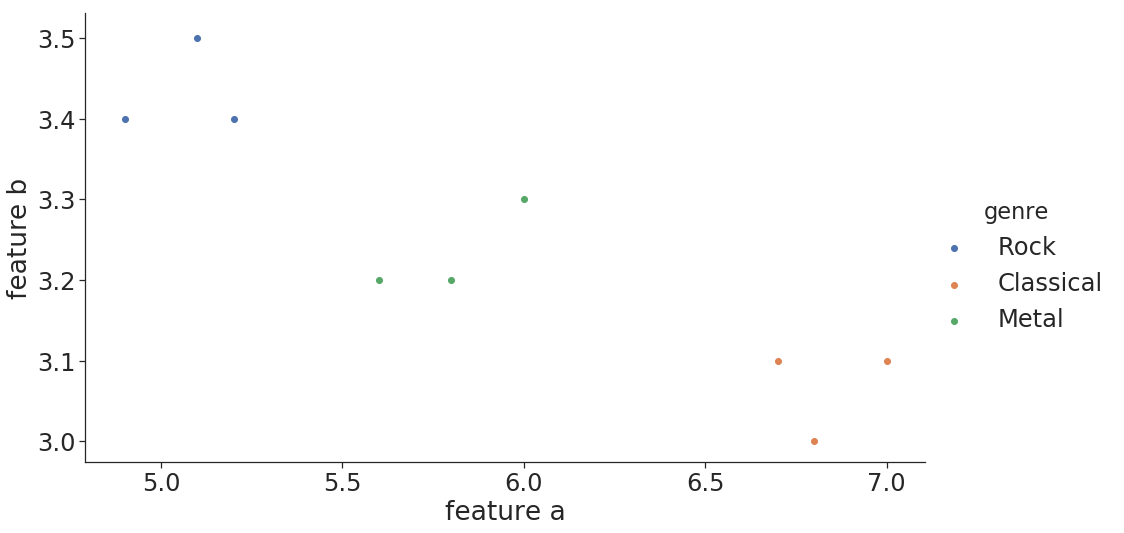
\includegraphics[scale=0.35]{Images/SparkFeat/featurespace.png}
		\captionof{figure}{Feature space example}
		\label{fig:featspace}
	}}
\end{figure}%
\FloatBarrier

\noindent The sampling of distances from different genres is vital for the analysis of the distribution of the distances, because the distances and their distribution vary, depending on where in the feature space the actual song is located. 
\noindent A song taken from the edge of the distribution of the feature space will end up with different distances than a song taken from the center. To visualize this, figure \ref{fig:featspace} shows a minimal example. While the distances from songs tagged with "Metal" to the songs tagged with "Rock" and "Classical" are about the same, the distances from a song taken off the Classical genre to the "Rock" or "Metal" songs are different in this example.\\ 
%For 95 song request that results in eight very large vectors containing the distances of song pairs. This large set of distances is then analyzed. 
\noindent Figure \ref{fig:corr2} shows the correlation between the distances from the various feature types. The eight different distances for each song pair are summed up into one new combined distance (following formula \ref{eq:distance} with all weights $w = 1$ ). This combined distance is labeled as "agg" in the following plots.

\begin{figure}[htbp]
	\centering
	\framebox{\parbox{1\textwidth}{ 			
			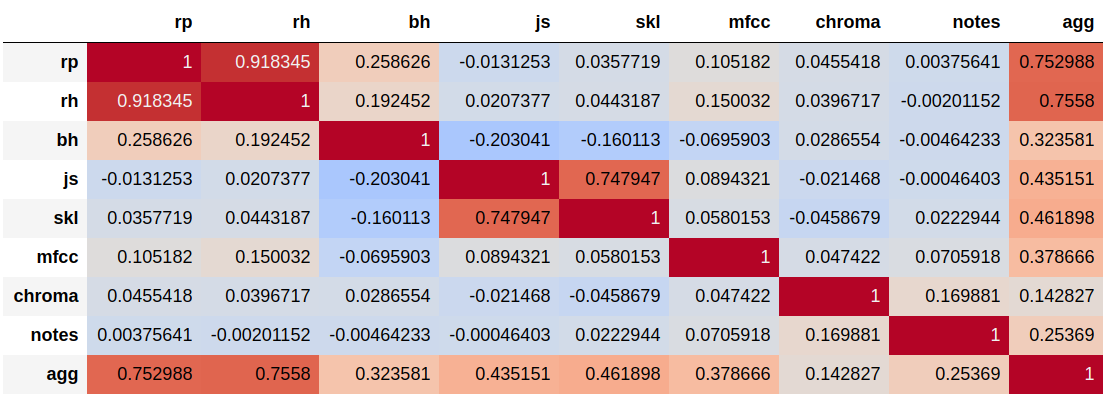
\includegraphics[scale=0.4]{Images/SparkFeat/corr_95_1517.png}	
	}}
	\caption{correlation 95 songs, 19 genres (5 each), 1517 artists}
	\label{fig:corr2}
\end{figure}\FloatBarrier

\noindent The correlation of a feature type with the overall distance is a sign of the impact of the feature type on the overall distance from the weighted sum. But because not all distances are equally distributed over the unit interval, the different feature types have different impacts on the sum of distances. This problem was already mentioned in section \ref{distsc} and section \ref{sparkskl}. Figure \ref{fig:cumdist} shows how the distances are distributed with the cumulative histograms over the unit interval. It is apparent that the cross-correlation distances are not evenly distributed. In section \ref{distsc}, a few proposals were already given how this problem could be solved in the future. 

\begin{figure}[htbp]
	\centering
	\framebox{\parbox{1\textwidth}{ 				
			\begin{subfigure}{.495\textwidth}
				\centering     
				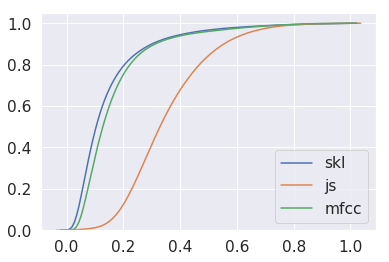
\includegraphics[scale=0.5]{Images/SparkFeat/cum1.png}
				\caption{cumulative distribution 1}
				\label{cum1}
			\end{subfigure}%	
			\begin{subfigure}{.495\textwidth}
				\centering    
				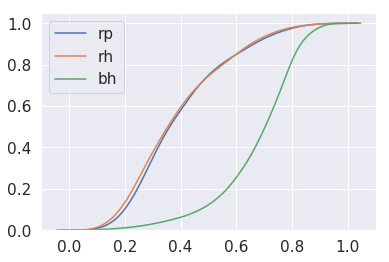
\includegraphics[scale=0.5]{Images/SparkFeat/cum2.png}
				\caption{cumulative distribution 2}
				\label{cum2}
			\end{subfigure}
			
			\begin{subfigure}{.495\textwidth}
				\centering     
				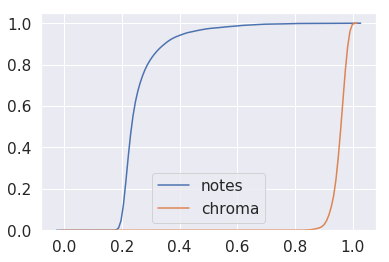
\includegraphics[scale=0.5]{Images/SparkFeat/cum3.png}
				\caption{cumulative distribution 3}
				\label{cum3}
			\end{subfigure}%		
			\begin{subfigure}{.495\textwidth}
				\centering    
				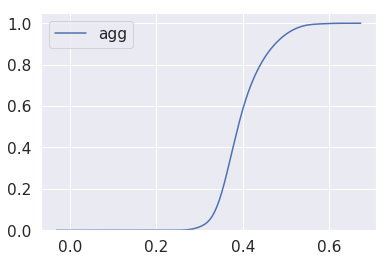
\includegraphics[scale=0.5]{Images/SparkFeat/cum4.png}
				\caption{cumulative distribution 4}
				\label{cum4}
			\end{subfigure}	
	}}
	\caption{Cumulative distributions}
	\label{fig:cumdist}
\end{figure}
\FloatBarrier

\noindent As mentioned in section \ref{sparkskl}, the SKL divergence was also prone to outliers and had issues when scaling distances to the unit interval. The solution was to filter out all song pairs with an SKL divergence larger than a certain threshold before scaling the distances. If this filter operation is left out nearly all distances calculated with the symmetric Kullback-Leibler divergence are close to zero after the scaling. The impact can be seen in figure \ref{fig:sklsc} and figure \ref{fig:corr}
\noindent If the outliers are not filtered, the correlation between the distances of the different feature types change drastically. The correlation of the unfiltered SKL distances with the combined distance ("agg") decreases significantly (see figure \ref{fig:corr}). Interestingly also the correlation of the Jensen-Shannon like divergence and the combined distance ("agg") is dropping. 

\begin{figure}[htbp]
	\centering
	\framebox{\parbox{1\textwidth}{ 
	\begin{subfigure}{0.5\textwidth}
		\centering
		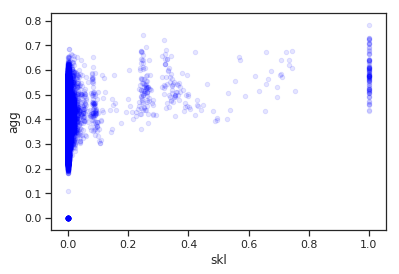
\includegraphics[scale=0.5]{Images/SparkFeat/skl_unscaled.png}
		\captionof{figure}{SKL unscaled}
		\label{scklusc}
	\end{subfigure}
	\begin{subfigure}{0.5\textwidth}
		\centering
		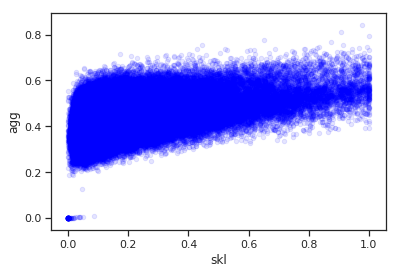
\includegraphics[scale=0.5]{Images/SparkFeat/skl_scaled.png}
		\captionof{figure}{SKL scaled}
		\label{scklsc}
	\end{subfigure}%
	}}
	\caption{Correlation of features depending on SKL scaling}
	\label{fig:sklsc}
\end{figure}
\FloatBarrier

\noindent A possible explanation could be that the SKL and JS distances are indeed highly correlated, but due to the bad scaling, the SKL has no impact on the overall distance. The results from the JS divergence alone are not able to impact the weighted sum of the combined distance in the same way both features together could. 

\begin{figure}[htbp]
	\centering
	\framebox{\parbox{1\textwidth}{
	\begin{subfigure}{0.5\textwidth}
		\centering
		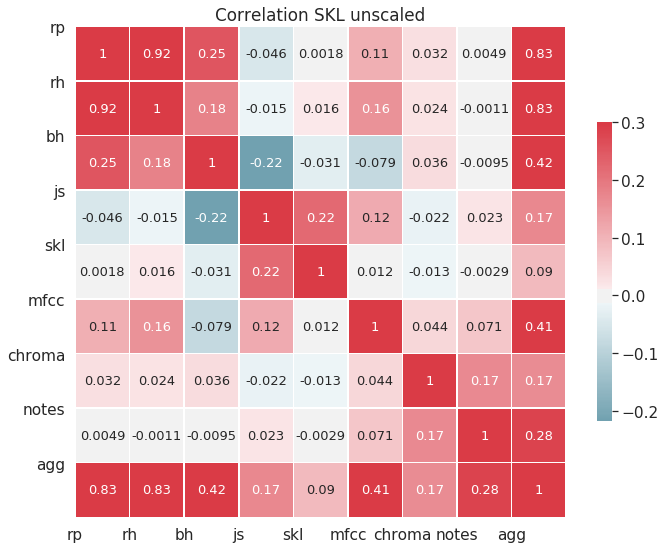
\includegraphics[scale=0.33]{Images/SparkFeat/skl_corr_unscaled.png}
		\captionof{figure}{SKL unscaled}
		\label{corrusc}
	\end{subfigure} 
	\begin{subfigure}{0.5\textwidth}
		\centering
		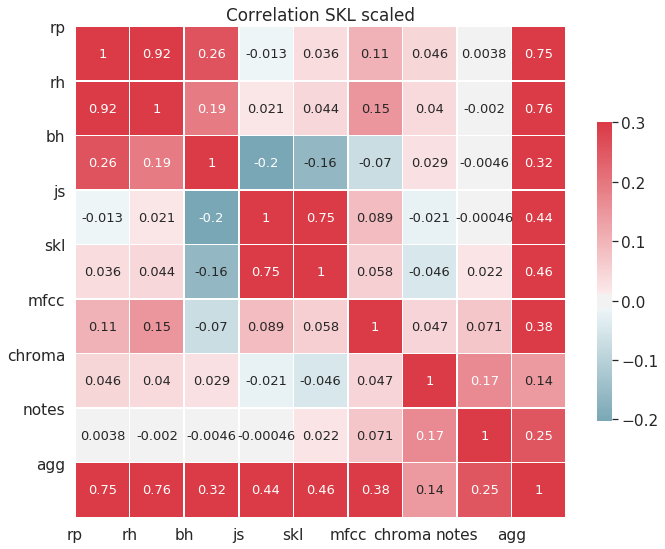
\includegraphics[scale=0.33]{Images/SparkFeat/skl_corr_scaled.png}
		\captionof{figure}{SKL scaled}
		\label{corrsc}
	\end{subfigure}%
	}}
	\caption{Correlation of features}
	\label{fig:corr}
\end{figure}
\FloatBarrier

\noindent The last plot (figure \ref{fig:corr3}) shows the full scatter matrix of the various distances. The main diagonal shows the histograms of the distances from the belonging unique feature-sets.

\begin{figure}[htbp]
	\centering
	\framebox{\parbox{1\textwidth}{	
	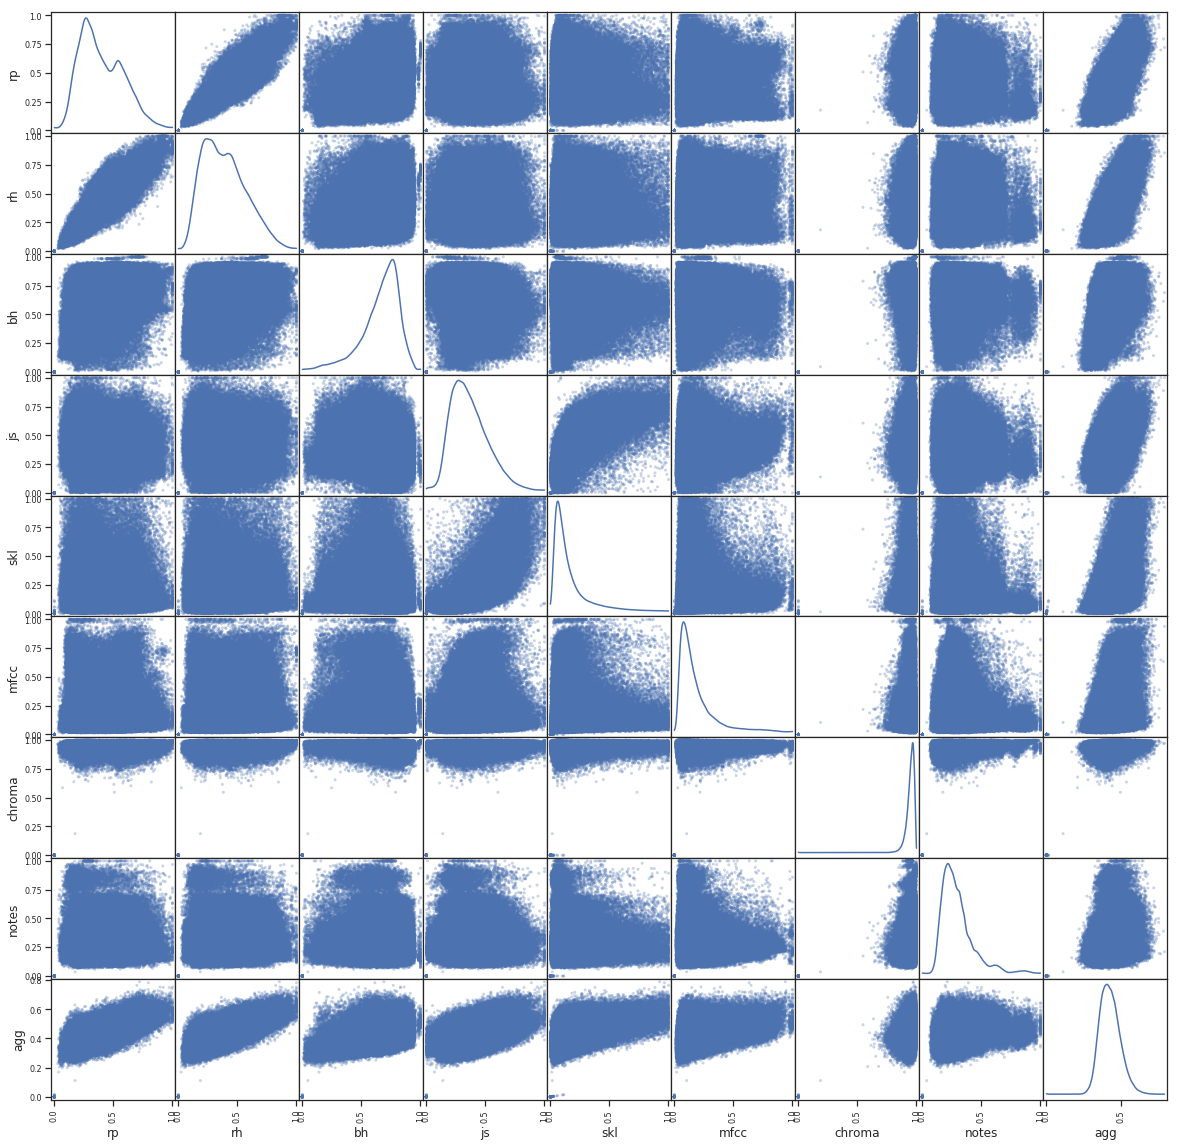
\includegraphics[scale=0.36]{Images/SparkFeat/scatter1517_KernelDensityEstimationHD.png}	
	\caption{correlation 95 songs, 19 genres (5 each), 1517 artists}
	\label{fig:corr3}
	}}
\end{figure}
\FloatBarrier

%\textit{\textbf{TODO: describe correlation of melodic features and AGG}}

\subsection{Cover Song Identification}\label{covsongid}

As mentioned in section \ref{covermfcc}, purely MFCC based recommender systems lack the ability to detect cover songs. Melody based similarity algorithms like the cross-correlation approach by Ellis and Poliner (see section \ref{crosscorrsec}) and the approach of using the Levenshtein distance by Xia (et al.) in section \ref{textretr}, on the other hand, were primarily implemented to detect cover songs. 


\begin{table}[H]
	\begin{minipage}{0.5\textwidth}
		\begin{center}
			\begin{tabular}{|l||c|}
				\hline
				chroma & 30\\
				\hline
				chroma + notes & 27\\
				\hline
				chroma + skl & 26\\
				\hline
				chroma + notes + rp & 24\\
				\hline
				chroma + rp & 22\\
				\hline
				chroma + skl + rp & 22\\
				\hline
				chroma + mfcc & 19\\
				\hline
				chroma + js + rp & 17\\
				\hline
				chroma + js & 17\\
				\hline
				notes & 17\\
				\hline
				chroma + mfcc + rp & 15\\
				\hline
				all & 15\\
				\hline
				notes + rp & 13\\
				\hline
				mfcc + notes + rp & 7\\
				\hline
				rp & 7\\
				\hline
				mfcc + js + skl & 3\\
				\hline
			\end{tabular}
		\end{center}
		\captionof{table}{Cover recognition - Top 1\label{cov_1}}
	\end{minipage}
	\begin{minipage}{0.5\textwidth}
		\begin{center}
			\begin{tabular}{|l||c|}
				\hline
				chroma & 33\\
				\hline
				chroma + notes & 31\\
				\hline
				chroma + notes + rp & 30\\
				\hline
				chroma + skl & 29\\
				\hline
				chroma + rp & 29\\
				\hline
				chroma + skl + rp & 26\\
				\hline
				chroma + mfcc + rp & 24\\
				\hline
				notes & 23\\
				\hline
				all & 23\\
				\hline
				chroma + mfcc & 22\\
				\hline
				chroma + js + rp & 22\\
				\hline
				chroma + js & 21\\
				\hline
				notes + rp & 19\\
				\hline
				rp & 15\\
				\hline
				mfcc + notes + rp & 14\\
				\hline
				mfcc + js + skl & 10\\
				\hline
			\end{tabular}
		\end{center}
		\captionof{table}{Cover recognition - Top 5\label{cov_2}}
	\end{minipage}
\end{table}

\noindent Running the first tests on the full dataset consisting of 114210 songs, the Spark implementation was able to find the cover of "Rock you like a Hurricane" by the Scorpions and covered by Knightsbridge as the top recommendation when using the cross-correlation.\\
\noindent The application was also able to find an alternative recording of the piece "Für Elise" cover as a top recommendation in over 114210 songs, even when using the filter and refine algorithm (starting with chroma features) presented in section \ref{farfs}.\\
\noindent As a third example the famous "Rondo Alla Turca (Allegretto)" also known as the Turkish March by Mozart was tested. This song was also used in chapter \ref{covermfcc} where the ability of the Musly toolkit to detect cover songs was tested. 
At first, a combination of js, chroma, and rp features was used. The top five results are listed below.\\
\ \\
\textit{\noindent Song request: 100 Meisterwerke der Klassik/ Mozart - Alla Turca (Allegretto) (private collection), JS + RP + CHROMA}

\begin{itemize}
	\setlength\itemsep{-0.5em}
	\item 1) Piano Perlen/ Mozart - Türkischer Marsch (private collection)
	\item 2) FRITZ STEINEGGER - RONDO ALLA TURCA KV 331 (1517 artists)
	\item 3) 136071 (fma dataset)
	\item 4) Sean Bennett - Variations on the Turkish March (1517 artists)
	\item 5) Mozart - Fantasie in D minor (1517 artists)
\end{itemize}

\noindent Two different versions were detected as the top results, and the fourth recommendation even listed a variation of the original song theme. Although the private music collection used contains two additional versions of this song (see section \ref{covermfcc}), the other versions could not be detected because the rp\_extract tool failed during the extraction of the features from these songs due to file format issues. So for the second attempt, the rhythm patterns were left out. The six top recommendations are again listed below:\\
\ \\
\textit{\noindent Song request: 100 Meisterwerke der Klassik/ Mozart - Alla Turca (Allegretto) (private collection), JS + CHROMA}

\begin{itemize}
	\setlength\itemsep{-0.5em}
	\item 1) Mozart Collection/ CD31/ KV331-3 Alla turca allegretto (private collection)
	\item 2) Piano Collection/ CD25 - Mozart - Alla Turca Allegretto (private collection)
	\item 3) Piano Perlen/ Mozart - Türkischer Marsch (private collection)
	\item 4) FRITZ STEINEGGER - RONDO ALLA TURCA KV 331 (1517 artists)
	\item 5) 136071 (2Kutup - We Shall Cuddle Up And Sleep) (fma dataset) 
	\item 6) Sean Bennett - Variations on the Turkish March (1517 artists)
\end{itemize}

\noindent Even if the JS features are left out and only the cross-correlation is computed, the top 6 results don't change. But on the other hand, even when the JS features are included, they aren't interfering with the cover song recognition. In a third request where only the Jensen-Shannon-like divergence was tested to detect the alternative recordings, the first version only appeared as the 13th recommendation. This confirmed the presumption that timbral features and the Jensen-Shannon-like divergence and the symmetric Kullback-Leibler divergence are not appropriate for cover song recognition.
\noindent But there are also song requests where the cross-correlation fails to detect the cover song, one example being the song Chandelier by Sia and the cover version by Pvris that was used in chapter \ref{chromafeat} to explain the computation of the chroma features.\\
\noindent To further quantify the ability to detect cover songs after the promising first tests, the covers80 dataset introduced in section \ref{cov801} was loaded onto the cluster. The 80 "A-versions" songs were passed to the Spark application as song requests, and the resulting nearest neighbors were analyzed. Table \ref{cov_1} counts the appearance of the "B-version" songs as the first recommendation while table \ref{cov_2} lists the count of the recommended cover versions in the top five results of the 80 requested songs when using different combinations of feature sets. As expected, the approaches using melodic similarity features perform best. The combination of the different timbre based features performs worst. Surprisingly the distances based on rhythm patterns are also able to detect cover songs.\\
\noindent Although 30 out of 80 on the first doesn't seem like a surprisingly good hit rate and is not quite as good as the results from the original paper, it has to be mentioned that most of the cover versions in the cover80 dataset differ a lot in musical style, instrumentation, rhythm and even genre from the original recordings. These differences in musical style were also mentioned in the original paper from Ellis and Cottin \cite[p. 3]{cover802}.
\noindent As an interesting side note, it has to be mentioned that the detected cover versions of the "chroma-" and "notes-only" requests were mostly the same. Besides two songs, the chroma feature cross-correlation approach detected all of the cover songs that the Levenshtein distance also detected. 

\subsection{Genre Similarity}\label{genrerec}

Another way to quantify the quality of the distances and therefore the quality of the music recommendations is to measure the genre recall rate. In a simple test on the 1517 artists dataset, five classical songs are passed to Spark, and the nearest neighbors based on the rhythm and timbre features (skl, js, mfcc, rp, rh, and bh) are calculated. Then the genres of the top ten recommendations from all five song requests are analyzed. The result is pictured in figure \ref{fig:genrerec}.  

\begin{figure}[htbp]
	\centering
	\framebox{\parbox{1\textwidth}{ 			
			\begin{subfigure}{.495\textwidth}
				\centering			
				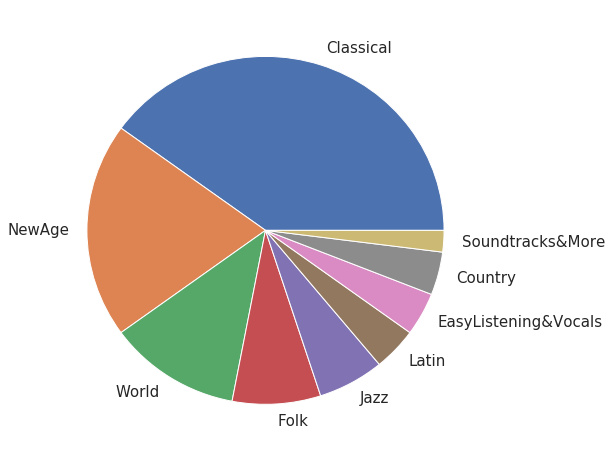
\includegraphics[scale=0.33]{Images/SparkFeat/1517clasall.png}
				\caption{1517 artist classical recommendations}
				\label{fig:genrerec}
			\end{subfigure}%	
			\begin{subfigure}{.495\textwidth}
				\centering			
				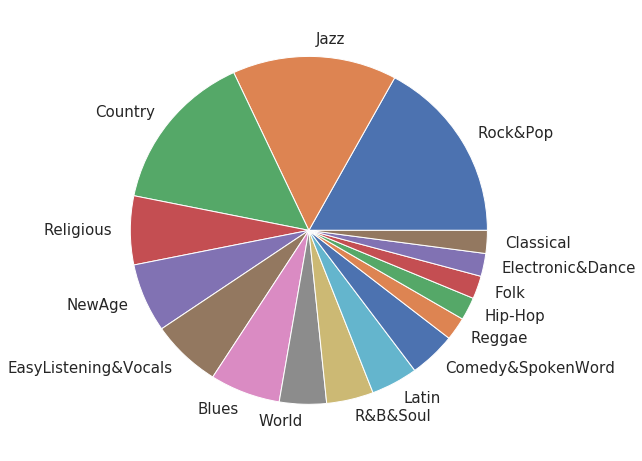
\includegraphics[scale=0.33]{Images/SparkFeat/1517rockall.png}
				\caption{1517 artist rock recommendations}
				\label{fig:genrerec2}
			\end{subfigure}		
	}}
	\caption{genre recall}
	\label{fig:1517gen}
\end{figure}
%\FloatBarrier

\noindent Although not all recommendations are classical songs, all recommended other genres like New Age, Wold, Folk and Jazz music are somewhat closely related to classical music.  Not a single song from more "modern" genres like Hip-Hop, Rock \& Pop, Electronic \& Dance or Reggae appears.
\noindent The same was tested with five songs from the Rock \& Pop genre (see figure \ref{fig:genrerec2}). The results are scattered across 16 out of 19 different genres from 1517 artists dataset. A possible explanation for this is, that the songs annotated with "Rock \& Pop" in this dataset come from a wider variety of sub-genres. When taking a closer look at the dataset, it shows that, e.g., also Metal songs are tagged as Rock \& Pop.\\
\begin{figure}[htbp]
	\centering
	\framebox{\parbox{1\textwidth}{ 			
			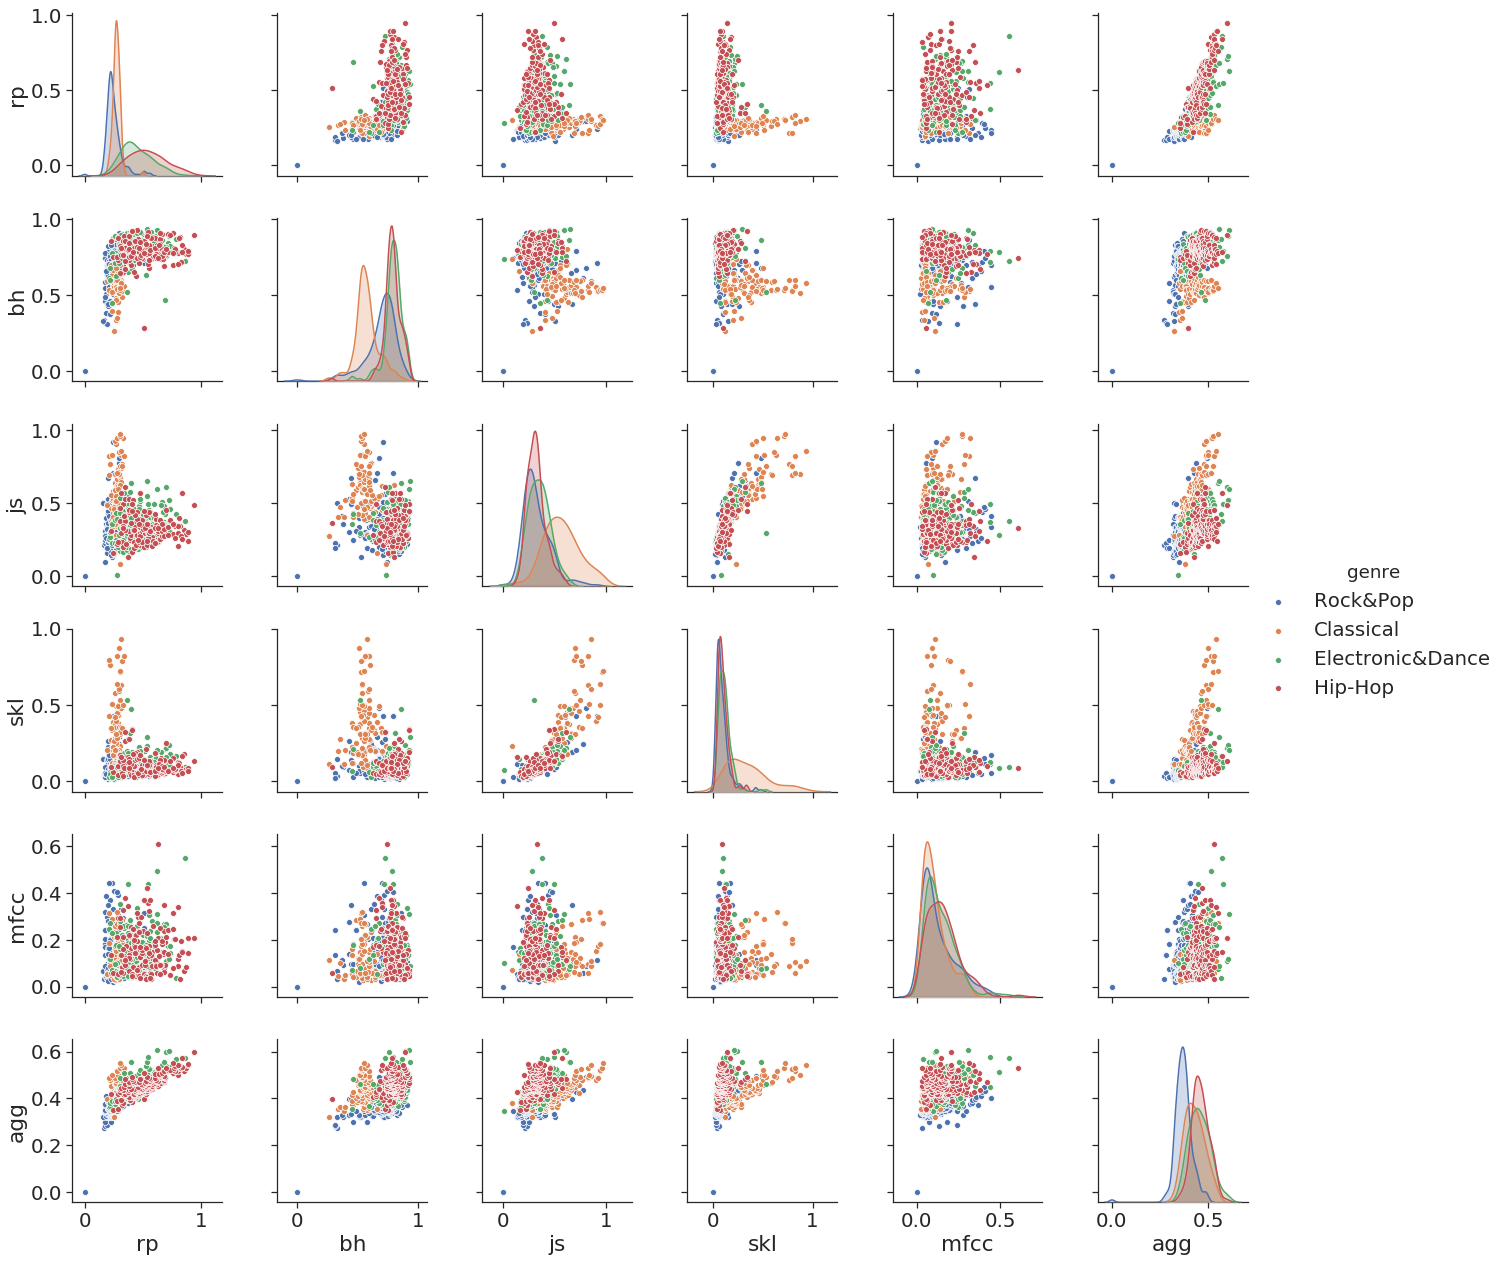
\includegraphics[scale=0.29]{Images/SparkFeat/rock.png}	
	}}
	\caption{distances 1 song, Rock\&Pop, 1517 artists, 4 genres}
	\label{fig:corr5}
\end{figure}
\FloatBarrier

\noindent To investigate the impact of different feature types on the overall recommendations and to visualize the distribution of distances for different genres, another test was performed. For single song requests, all distances to the songs from a subset of the 1517 artists dataset containing the genres "classical music", "hip-hop", "electronic \& dance" and "rock \& pop" were computed. Figure \ref{fig:corr5} shows the scatter matrices of all distances from one song request from the genre Rock \& Pop. The different distances of the recommendations are colored by the genre of the recommended song. 
\noindent On the main diagonal the Kernel Density Estimation of the respective feature-type is shown. One interesting detail that should be pointed out is that the JS distance alone is unable to distinguish between Rock/Pop songs and Hip-Hop songs but is able to separate between classical music and the rest. On the other hand, the rhythm patterns alone can't separate classical music from Rock/Pop. But when both feature-types are combined, all three genres can be separated. The scatter plot of the distances from the Rhythm Patterns and Jensen-Shannon-like divergence in combination shows three clusters of songs belonging to different genres. The fourth genre, "Electronic \& Dance" however can not be separated from Hip-Hop songs no matter what feature-set is used. But it has to be kept in mind that all these distances are distances between a song request from the Rock/Pop genre. 

\begin{figure}[htbp]
	\centering
	\framebox{\parbox{1\textwidth}{ 			
			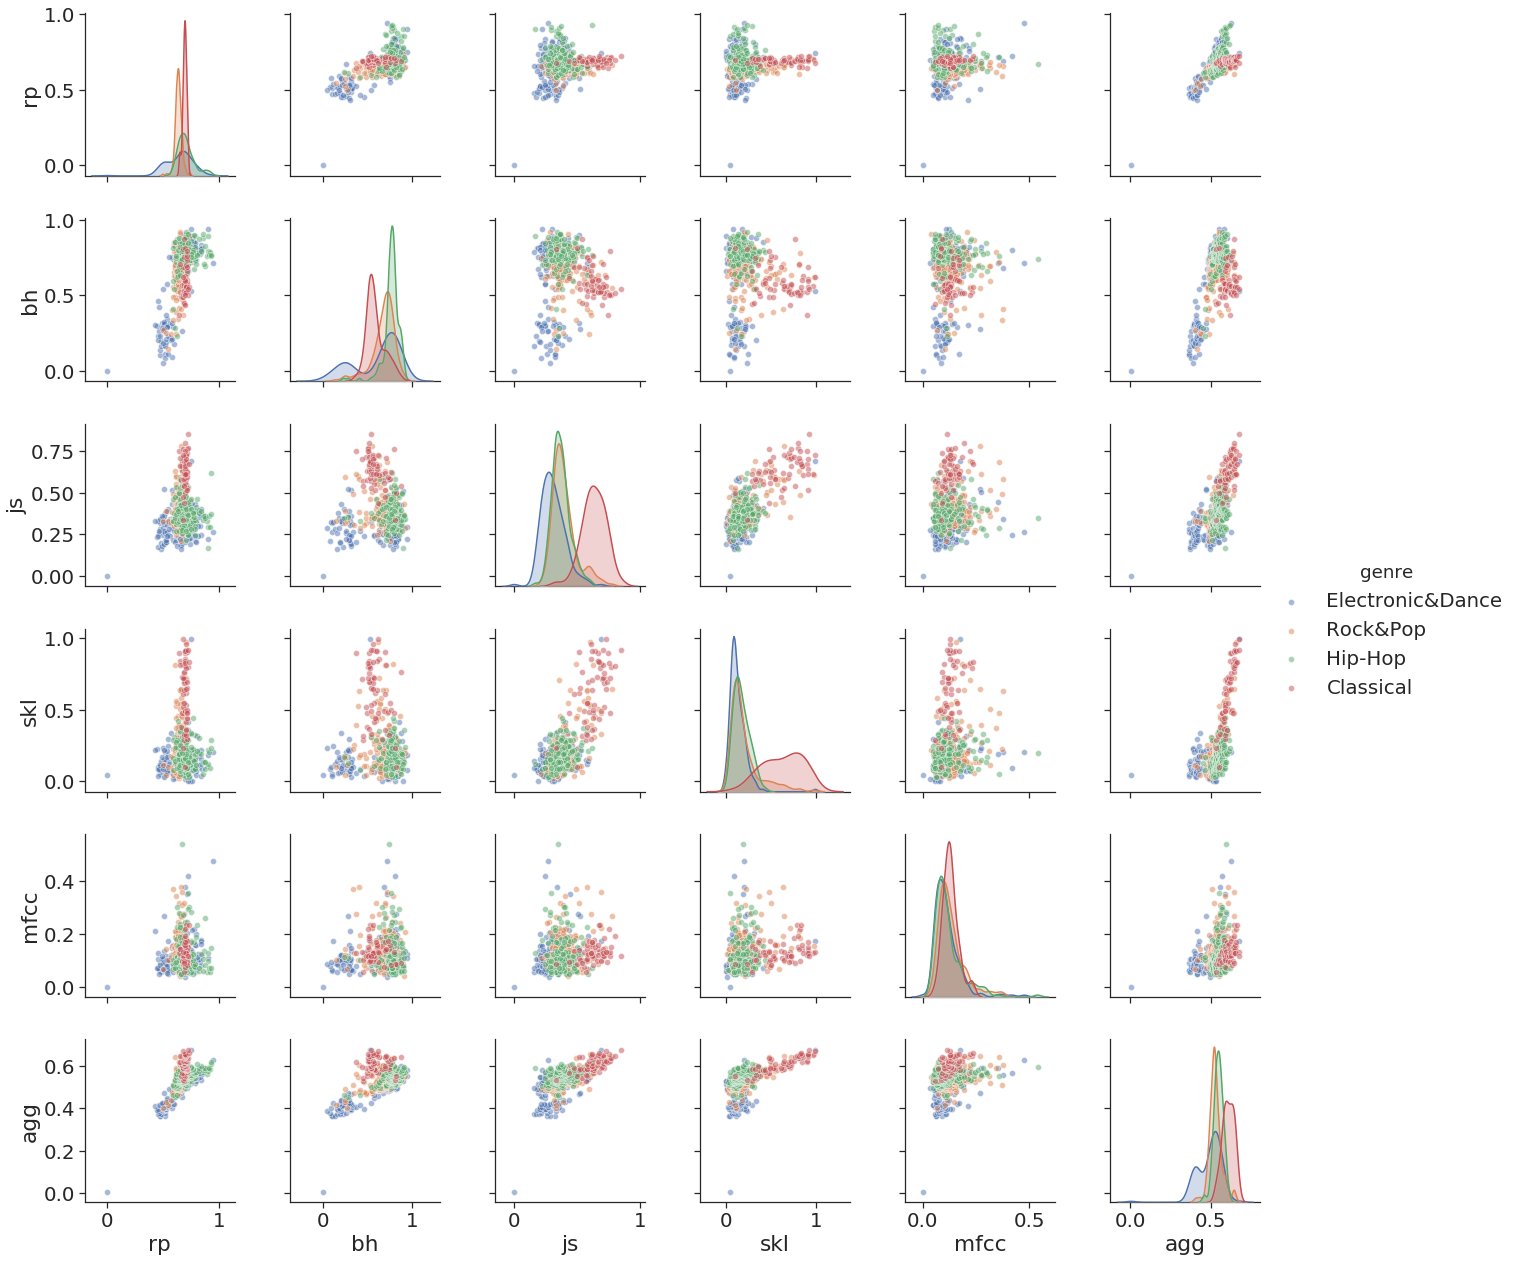
\includegraphics[scale=0.29]{Images/SparkFeat/electronic.png}	
	}}
	\caption{distances 1 song, electronic, 1517 artists, 4 genres}
	\label{fig:corr6}
\end{figure}
\FloatBarrier

\noindent As mentioned in section \ref{featqual} and visualized in figure \ref{fig:featspace}, the distribution of the distances varies depending on where in the feature space the song request is located. Apparently the songs of the Hip-Hop and Electronic/Dance genre are on average all about the same distance away from the requested Rock/Pop song. When requesting a song from the genre Electronic/Dance, the distribution of the distances look entirely different (see figure \ref{fig:corr6}).
\noindent The "agg" - plots represent the weighted sum of all features combined (also including cross-correlation and Levenshtein distances not shown in the plots). After the combination of all feature-types, the returned results primarily recommend other Rock \& Pop songs in figure \ref{fig:corr5} and Electronic \& Dance songs in figure \ref{fig:corr6}.\\
When using only one feature set, the Spark recommendation engine would not be able to separate all four of the different genres from each other. Only due to the combination of different rhythmic and timbral features an overall satisfying list of recommendations can be returned.\\

\subsection{Rhythm Features}\label{rhythmrec}

\begin{figure}[htbp]
	\centering
	\framebox{\parbox{1\textwidth}{ 			
			\begin{subfigure}{.495\textwidth}
				\centering			
				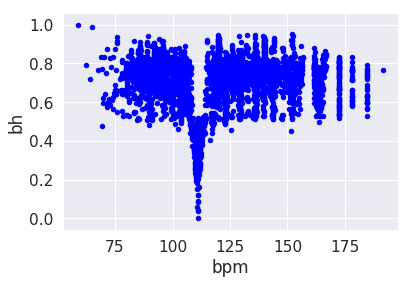
\includegraphics[scale=0.5]{Images/SparkFeat/BH_BPM.png}	
				\caption{BPM - BH (Rock\&Pop)}
				\label{fig:bbpm}
			\end{subfigure}		
			\begin{subfigure}{.495\textwidth}
				\centering			
				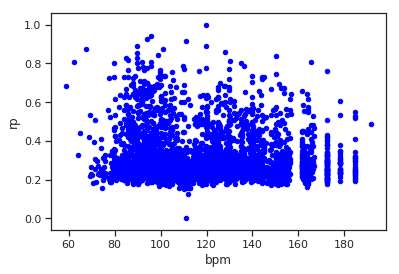
\includegraphics[scale=0.5]{Images/SparkFeat/RP_BPM.png}	
				\caption{BPM - RP (Rock\&Pop)}
				\label{fig:rbpm}
			\end{subfigure}%	
			
			\begin{subfigure}{.495\textwidth}
				\centering			
				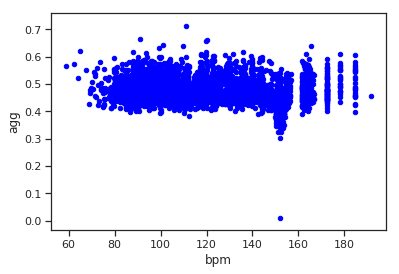
\includegraphics[scale=0.5]{Images/SparkFeat/bpm_agg_hip.png}	
				\caption{BPM - AGG (Rock\&Pop)}
				\label{fig:arbpm}
			\end{subfigure}		
			\begin{subfigure}{.495\textwidth}
				\centering			
				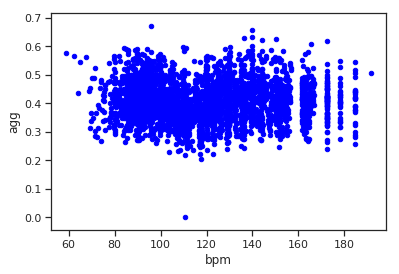
\includegraphics[scale=0.5]{Images/SparkFeat/bpm_agg_clas.png}	
				\caption{BPM - AGG (Classical)}
				\label{fig:acbpm}
			\end{subfigure}%			
	}}
	\caption{Rhythm features/ BPM}
	\label{fig:rhythmfeat}
\end{figure}
\FloatBarrier

\noindent Another critical requirement for the recommendation engine is the ability to return songs that are about the same tempo. To investigate the capabilities of the rhythm features, figure \ref{fig:rhythmfeat} shows the resulting distances of two song requests performed on the 1517 artists dataset.
\noindent The scatter plots show that the beat histogram and the rhythm patterns are closely related to the overall BPM of the songs. The "agg" value (the weighted sum) includes all eight different feature types, so the overall impact of the rhythm features on the recommendations can be seen. All in all, the Spark recommendation engine is more likely to recommend songs that have similar BPM when rhythm features are included in the weighted sum. The classical song request in figure \ref{fig:acbpm} also shows that the overall distances still are not exclusively dominated by the bpm but rather slightly influenced. 

\section{Subjective Evaluation}

This section includes the personal opinion and music taste of the author. Although these results are not "scientific", music taste is something personal and judging music recommendation solely from an objective perspective would be the wrong approach. The core strength of this Spark-based recommender system is that its parameters can be used to personalize the music recommendation. 

\subsection{Beyond Genre Boundaries}

The main reason for the choice of the topic of this thesis was that recommender systems as they come with streaming platforms like Spotify tend to value. For example, the "Song Radio"- option coming with Spotify stays in the boundaries of genres and is heavily influenced by other peoples listening behavior. Although this is not necessarily a bad thing, this thesis tried to focus directly on the tonal, rhythmic, and melodic properties. As a result, songs from other genres are recommended as can be seen in the following example. 
\noindent When searching for the nearest neighbors of the "Prelude in C- Sharp Minor (Op. 3 No. 2)" by the Russian composer Sergei Rachmaninoff based on the euclidean distance of MFCCs, the following results were returned: 

\begin{itemize}
	\setlength\itemsep{-0.5em}
	\item Klassik/Rachmaninoff - Piano Concerto No2 In C Minor Op18-1 Moderato
	\item Klassik/Liszt - Piano Concerto No 1 in E flat major S124(LWH4) Allegro maestoso
	\item Klassik/Brahms - Piano Sonata No2 in F sharp minor Op2 - III Scherzo allegro
	\item \underline{Metal\&Rock/Steve Moore - Intro \& Credits}
	\item Klassik/Liszt - Piano Concerto No 1 in E flat major S124(LWH4) Allegro animato
\end{itemize}

\noindent The "Metal \& Rock" recommendation seems out of place at first glance, but when taking a closer look, the recommended song is called "Intro \& Credits". When listening to it, some similarities are recognizable; it is a calm, dark instrumental piece made of synthesizer sounds. The original requested Prelude is a dark piano piece. Of course, this is just one example, and the recommendation is arguably not perfect. In general some of the timbre based recommendations seen out of place. This might be due to the choice of 13 MFCC bands over 25 as the musly toolkit uses, or maybe there are some unnoticed issues with the implementation left, which would have to be investigated in future work. But as also stated in section \ref{genrerec}, the overall performance concerning the genre recall rate is reasonably good.

\subsection{Personal Music Taste}\label{personal}

As a last side note on personal music taste, a test using one of my favorite songs was made. As already mentioned, my private music collection was a part of this thesis. To retain some kind of reproducibility the whole collection is documented, and the according list of albums and songs is on a document on the CD in the appendix. On the last pages of this document, there is also a list containing my personal song favorites in the metal music genre. One of these songs was chosen, and the recommendations based on rhythm patterns were calculated for the private music collection. The song is called "The Art Of Dying" by the band Gojira. The recommendations are listed below. Another track from my personal list of favorite song appears as a recommendation. 

\begin{itemize}
	\setlength\itemsep{-0.5em}
	\item Numenorean - Adore
	\item Shylmagoghnar - Transience
	\item \underline{Amon Amarth - The Last Stand Of Frej}
	\item Delain - We Are the Others
	\item Ensiferum - Descendants Defiance Domination
\end{itemize}

\noindent This could be an indication that my taste in music is closely related to the rhythmic properties of the music. 
An idea for future research could be to reverse engineer a user's musical taste by looking at a list of favorite songs. The information which songs a user likes the most is already available to all streaming platforms because most likely the songs a user listens to the most are also the songs he likes the best. Spark could be used to calculate the similarities between these favorite songs of a user and analyze the distances. Whether or not these songs are more similar in rhythm, melody or timbre could enhance the parametrization of a recommender engine and further personalize music recommendations by adapting the weights of a recommendation engine.\\
Of course, the field of personalized music recommendation is an already existing one, but maybe the addition of Spark and big data opportunities of using audio content instead of contextual information and collaborative filtering could enhance these existing systems. 

\chapter{Summary}

\section{Conclusion}

Looking back at the content of this thesis, the first chapter provided an overview of the field of music information retrieval. Different high- and low-level audio features were explained, and various ways to measure the similarities between audio files based on the audio features were introduced. Additionally, a short introduction to Big Data frameworks, especially Apache Spark and Hadoop was given, and different audio data sources were gathered. The second chapter presented ways to extract and pre-process timbre, rhythm, and melodic features from audio files and multiple algorithms for calculating the distances between the extracted features were given. With the theoretic knowledge from the first chapters, the implementation could be planned. The data was collected. Over 1TB of music files containing 114000 different songs were aggregated.\\ 
In the first part of the implementation the necessary audio features were extracted and pre-processed (e.g., by extracting the melody estimation) in parallel using MPI on a computer cluster, paving the way for the usage with the Big Data processing framework Spark.
The features were loaded into the HDFS of a cluster and multiple similarity measurements were implemented, tested, evaluated, and improved using the Spark framework. With Spark, multiple approaches (RDD, DataSet, Filter and Refine, Cluster Configurations) were implemented, tested, and the runtime was measured. The resulting distances presented, analyzed, and visualized.\\
\ \\
The final application is able to recommend songs similar to a song request by computing the distances. The recommendations are parameterized, giving the user the option to prioritize different aspects of the music. The system is scalable. More songs can be added, the cluster size can be increased, and the possibility to add different kinds of audio features and more state-of-the-art similarity measurements is also given. 

\section{Outlook}

There are still a few minor flaws, especially when looking at the implementation of the symmetric Kullback-Leibler divergence and the Jensen-Shannon divergence and the scaling of the distances. The different starting points for possible future research were laid out during the whole thesis and are summarized here.\\
First of all the file format issues with *.wav audio files when using the rp\_extract tool from the TU Wien should be fixed to be able to compute all features from all the songs of a dataset (see section \ref{totamsong}).\\
The next step would be to re-evaluate the Jensen-Shannon-like divergence and the symmetric Kullback-Leibler divergence and fix the issues with the outliers. Also, the issues with non-invertible or non-singular covariance matrices should be investigated (see section \ref{sparkskl} and \ref{jsld}). Maybe also the proposed enhancements by Schnitzer \cite{schnitzer1} of reducing the hubness with mutual proximity and by using more MFCC bands would be sufficient to improve the quality of the recommendations (see section \ref{mprox}). The scaling of the different features could be improved in a way, where all feature are evenly distributed over the unit interval (see section \ref{distsc}).\\
Tests of the performance on larger clusters and with more data would be critical to assess the scaling of the problem.
An implementation of the Spark streaming abilities to enable real-time computation of similarities instead of using batch-processing job would be the next logical step if the goal is to develop a system able to run with music streaming platforms. When evaluating the genre recall rate with Spark, an issue with the garbage collection running out of memory after 40 subsequent song requests was encountered and should be fixed first.\\
\noindent As another way of improving the presented Spark application, more state of the art similarity measurements like block-level features (section \ref{blocklevel}) or the TF-IDF weights (section \ref{textretr}) for melodic similarity could be added. The most promising enhancement for the developed recommendation engine in this thesis would be the addition of genre and metadata information, genre specific features, collaborative filtering, and lyrics (see section \ref{collaborative}). All the contextual music information that would typically be processed by a Big Data framework wasn't included in this thesis but could significantly enhance the recommendations. Most streaming services already have all the information to add available, like users listening behavior or audio metadata and services like Spotify are also already using Spark for collaborative filtering so the Spark application presented in this thesis could be added and integrated into running streaming systems.\\
A last suggestion for future enhancements is to investigate the proposal from section \ref{personal} of personalized music recommendation based on the audio feature similarities of a user's favorite songs made available by the Big Data framework.

%\addtolength{\textheight}{-12cm}   % This command serves to balance the column lengths
% on the last page of the document manually. It shortens
% the textheight of the last page by a suitable amount.
% This command does not take effect until the next page
% so it should come on the page before the last. Make
% sure that you do not shorten the textheight too much.